\documentclass[aspectratio=169]{beamer}

\usetheme{Madrid}

% ---- SCIP blue color scheme --------------------------------
\definecolor{scipblue}{RGB}{30,60,190}
\setbeamercolor{structure}{fg=scipblue}
\setbeamercolor{palette primary}{bg=scipblue, fg=white}
\setbeamercolor{palette secondary}{bg=scipblue!85!black, fg=white}
\setbeamercolor{palette tertiary}{bg=scipblue!70!black, fg=white}
\setbeamercolor{palette quaternary}{bg=scipblue, fg=white}
\setbeamercolor{frametitle}{bg=scipblue!10, fg=scipblue}
\setbeamercolor{title}{fg=white, bg=scipblue}
\setbeamercolor{item}{fg=scipblue}

\usepackage{amsmath, amssymb}
\usepackage{tikz}
\usetikzlibrary{arrows.meta, positioning, shapes.geometric, fit, decorations.pathreplacing, calc}
\usepackage{booktabs}
\usepackage{listings}
\usepackage{hyperref}

\lstset{
  language=Python,
  basicstyle=\ttfamily\scriptsize,
  keywordstyle=\color{blue!70!black}\bfseries,
  commentstyle=\color{green!50!black}\itshape,
  stringstyle=\color{red!60!black},
  showstringspaces=false,
  breaklines=true,
  frame=single,
  columns=fullflexible,
  morekeywords={Model, quicksum, Pricer, Branchrule, Conshdlr, Sepa}
}

\title{APDIO Workshop: Optimization Software \& Practice}
\subtitle{Part 3: Branch-and-Price}
\author{Jo\~{a}o Dion\'{i}sio}
\date{March 27, 2026}
\titlegraphic{%
  
\includegraphics[height=0.6cm]{media/uporto_logo.jpg}\hspace{1.5cm}%
  
\includegraphics[height=1.5cm]{media/sciplogo.png}\hspace{1.5cm}%
  
\includegraphics[height=1.0cm]{media/apdio_logo.png}%
}

\begin{document}

% ---------------------------------------------------------
% Frame 1: Title
% ---------------------------------------------------------
\begin{frame}
\titlepage
\end{frame}

% ---------------------------------------------------------
% Frame 2: Roadmap
% ---------------------------------------------------------
\begin{frame}{Roadmap}
\begin{center}
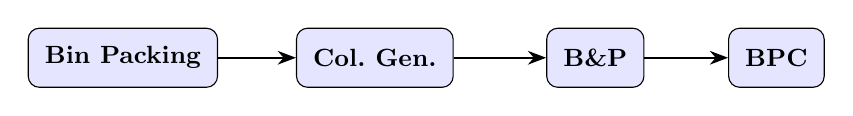
\begin{tikzpicture}[
  box/.style={draw, rounded corners, fill=blue!10,
              minimum height=0.75cm, font=\small\bfseries, inner xsep=6pt},
  arr/.style={-{Stealth}, thick}
]
  \node[box] (bpp) at (0, 0)   {Bin Packing};
  \node[box] (cg)  at (3.2, 0) {Col.\ Gen.};
  \node[box] (bp)  at (6.0, 0) {B\&P};
  \node[box] (bpc) at (8.3, 0) {BPC};

  \draw[arr] (bpp) -- (cg);
  \draw[arr] (cg)  -- (bp);
  \draw[arr] (bp)  -- (bpc);
\end{tikzpicture}
\end{center}

\medskip
\begin{itemize}
  \item \textbf{Column generation:} add \textbf{variables} dynamically (dual of row generation)
  \item \textbf{Branch-and-price:} column generation inside branch-and-bound
  \item \textbf{Branch-price-and-cut:} add cutting planes on top
  \item \textbf{Application:} Bin Packing Problem
\end{itemize}
\end{frame}

% ---------------------------------------------------------
% Frame 3: Bin Packing Problem
% ---------------------------------------------------------
\begin{frame}{Bin Packing Problem}
\begin{columns}[T]
\begin{column}{0.52\textwidth}
\textbf{Given:} items with sizes $s_i$, bins with capacity $C$

\textbf{Goal:} pack all items using the fewest bins

\medskip
\begin{itemize}
  \item NP-hard; applications in logistics, scheduling, cloud computing
  \item We will explore two formulations:
    \begin{enumerate}
      \item Compact (assignment variables) --- symmetry, weak LP
      \item Extended (pattern variables) --- column generation
    \end{enumerate}
\end{itemize}
\end{column}
\begin{column}{0.45\textwidth}
\centering
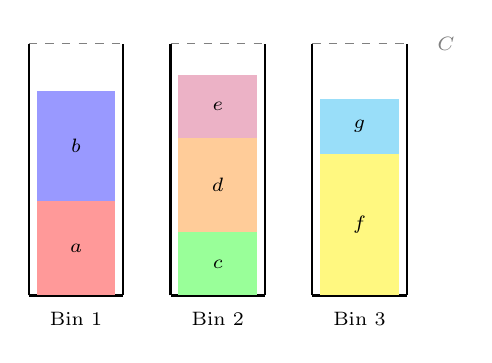
\begin{tikzpicture}[
  bin/.style={draw, thick, minimum width=1.2cm},
  item/.style={draw, minimum width=1cm, font=\scriptsize\bfseries,
               align=center}
]
  % Capacity line height
  \def\caph{3.2}

  % Bin 1
  \draw[thick] (0,0) -- (0,\caph) (1.2,0) -- (1.2,\caph);
  \draw[thick] (0,0) -- (1.2,0);
  \fill[red!40] (0.1,0) rectangle (1.1, 1.2);
  \node[font=\scriptsize\bfseries] at (0.6, 0.6) {$a$};
  \fill[blue!40] (0.1,1.2) rectangle (1.1, 2.6);
  \node[font=\scriptsize\bfseries] at (0.6, 1.9) {$b$};
  \draw[dashed, gray] (0, \caph) -- (1.2, \caph);
  \node[font=\scriptsize] at (0.6, -0.3) {Bin 1};

  % Bin 2
  \draw[thick] (1.8,0) -- (1.8,\caph) (3.0,0) -- (3.0,\caph);
  \draw[thick] (1.8,0) -- (3.0,0);
  \fill[green!40] (1.9,0) rectangle (2.9, 0.8);
  \node[font=\scriptsize\bfseries] at (2.4, 0.4) {$c$};
  \fill[orange!40] (1.9,0.8) rectangle (2.9, 2.0);
  \node[font=\scriptsize\bfseries] at (2.4, 1.4) {$d$};
  \fill[purple!30] (1.9,2.0) rectangle (2.9, 2.8);
  \node[font=\scriptsize\bfseries] at (2.4, 2.4) {$e$};
  \draw[dashed, gray] (1.8, \caph) -- (3.0, \caph);
  \node[font=\scriptsize] at (2.4, -0.3) {Bin 2};

  % Bin 3
  \draw[thick] (3.6,0) -- (3.6,\caph) (4.8,0) -- (4.8,\caph);
  \draw[thick] (3.6,0) -- (4.8,0);
  \fill[yellow!50] (3.7,0) rectangle (4.7, 1.8);
  \node[font=\scriptsize\bfseries] at (4.2, 0.9) {$f$};
  \fill[cyan!40] (3.7,1.8) rectangle (4.7, 2.5);
  \node[font=\scriptsize\bfseries] at (4.2, 2.15) {$g$};
  \draw[dashed, gray] (3.6, \caph) -- (4.8, \caph);
  \node[font=\scriptsize] at (4.2, -0.3) {Bin 3};

  % Capacity label
  \node[font=\scriptsize, gray] at (5.3, \caph) {$C$};
\end{tikzpicture}
\end{column}
\end{columns}
\end{frame}

% ---------------------------------------------------------
% Frame 4: Compact Formulation
% ---------------------------------------------------------
\begin{frame}{Compact Formulation}
\textbf{Variables:} $x_{ib} \in \{0,1\}$ (item $i$ in bin $b$),
$y_b \in \{0,1\}$ (bin $b$ used)

\begin{align*}
  \min \quad & \sum_{b} y_b \\
  \text{s.t.} \quad
    & \sum_{b} x_{ib} = 1 && \forall\, i \quad \text{(assign each item)} \\
    & \sum_{i} s_i\, x_{ib} \le C\, y_b && \forall\, b \quad \text{(capacity)} \\
    & x_{ib}, y_b \in \{0,1\}
\end{align*}

\begin{center}
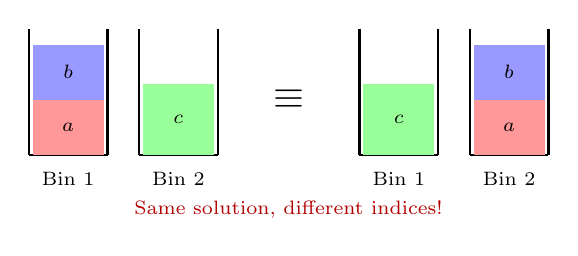
\begin{tikzpicture}[
  item/.style={draw, minimum width=0.7cm, font=\scriptsize\bfseries, align=center}
]
  % Bin A (left)
  \draw[thick] (0,0) -- (0,1.6) (1.0,0) -- (1.0,1.6);
  \draw[thick] (0,0) -- (1.0,0);
  \fill[red!40] (0.05,0) rectangle (0.95, 0.7);
  \node[font=\scriptsize\bfseries] at (0.5, 0.35) {$a$};
  \fill[blue!40] (0.05,0.7) rectangle (0.95, 1.4);
  \node[font=\scriptsize\bfseries] at (0.5, 1.05) {$b$};
  \node[font=\scriptsize] at (0.5, -0.3) {Bin 1};

  % Bin B (left)
  \draw[thick] (1.4,0) -- (1.4,1.6) (2.4,0) -- (2.4,1.6);
  \draw[thick] (1.4,0) -- (2.4,0);
  \fill[green!40] (1.45,0) rectangle (2.35, 0.9);
  \node[font=\scriptsize\bfseries] at (1.9, 0.45) {$c$};
  \node[font=\scriptsize] at (1.9, -0.3) {Bin 2};

  % Equivalence symbol
  \node[font=\Large\bfseries] at (3.3, 0.7) {$\equiv$};

  % Bin A (right -- swapped)
  \draw[thick] (4.2,0) -- (4.2,1.6) (5.2,0) -- (5.2,1.6);
  \draw[thick] (4.2,0) -- (5.2,0);
  \fill[green!40] (4.25,0) rectangle (5.15, 0.9);
  \node[font=\scriptsize\bfseries] at (4.7, 0.45) {$c$};
  \node[font=\scriptsize] at (4.7, -0.3) {Bin 1};

  % Bin B (right -- swapped)
  \draw[thick] (5.6,0) -- (5.6,1.6) (6.6,0) -- (6.6,1.6);
  \draw[thick] (5.6,0) -- (6.6,0);
  \fill[red!40] (5.65,0) rectangle (6.55, 0.7);
  \node[font=\scriptsize\bfseries] at (6.1, 0.35) {$a$};
  \fill[blue!40] (5.65,0.7) rectangle (6.55, 1.4);
  \node[font=\scriptsize\bfseries] at (6.1, 1.05) {$b$};
  \node[font=\scriptsize] at (6.1, -0.3) {Bin 2};

  % Annotation
  \node[font=\scriptsize, text=red!70!black] at (3.3, -0.7)
    {Same solution, different indices!};
\end{tikzpicture}
\end{center}

\vspace{-0.2cm}
\begin{itemize}
  \item \textbf{Enormous symmetry}: permuting bin indices $\Rightarrow$ equivalent solutions
  \item \textbf{Weak LP relaxation}: impractical for large instances
\end{itemize}
\end{frame}

% ---------------------------------------------------------
% Frame 5: Modeling with Patterns
% ---------------------------------------------------------
\begin{frame}{A Different Perspective: Patterns}
Instead of deciding \emph{where each item goes}, let's think about
all the ways a single bin can be packed --- \textbf{patterns} (or packings).

\medskip
\begin{center}
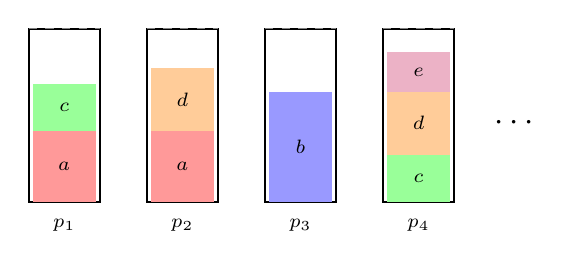
\begin{tikzpicture}[
  bin/.style={draw, thick, minimum width=1cm},
  item/.style={font=\scriptsize\bfseries}
]
  \def\caph{2.2}
  \def\bw{0.9}

  % Pattern 1: {a,c}
  \draw[thick] (0,0) rectangle (\bw,\caph);
  \fill[red!40] (0.05,0) rectangle (0.85, 0.9);
  \node[item] at (0.45, 0.45) {$a$};
  \fill[green!40] (0.05,0.9) rectangle (0.85, 1.5);
  \node[item] at (0.45, 1.2) {$c$};
  \draw[dashed, gray] (0,\caph) -- (\bw,\caph);
  \node[font=\scriptsize] at (0.45, -0.3) {$p_1$};

  % Pattern 2: {a,d}
  \draw[thick] (1.5,0) rectangle (1.5+\bw,\caph);
  \fill[red!40] (1.55,0) rectangle (2.35, 0.9);
  \node[item] at (1.95, 0.45) {$a$};
  \fill[orange!40] (1.55,0.9) rectangle (2.35, 1.7);
  \node[item] at (1.95, 1.3) {$d$};
  \draw[dashed, gray] (1.5,\caph) -- (1.5+\bw,\caph);
  \node[font=\scriptsize] at (1.95, -0.3) {$p_2$};

  % Pattern 3: {b}
  \draw[thick] (3.0,0) rectangle (3.0+\bw,\caph);
  \fill[blue!40] (3.05,0) rectangle (3.85, 1.4);
  \node[item] at (3.45, 0.7) {$b$};
  \draw[dashed, gray] (3.0,\caph) -- (3.0+\bw,\caph);
  \node[font=\scriptsize] at (3.45, -0.3) {$p_3$};

  % Pattern 4: {c,d,e}
  \draw[thick] (4.5,0) rectangle (4.5+\bw,\caph);
  \fill[green!40] (4.55,0) rectangle (5.35, 0.6);
  \node[item] at (4.95, 0.3) {$c$};
  \fill[orange!40] (4.55,0.6) rectangle (5.35, 1.4);
  \node[item] at (4.95, 1.0) {$d$};
  \fill[purple!30] (4.55,1.4) rectangle (5.35, 1.9);
  \node[item] at (4.95, 1.65) {$e$};
  \draw[dashed, gray] (4.5,\caph) -- (4.5+\bw,\caph);
  \node[font=\scriptsize] at (4.95, -0.3) {$p_4$};

  % Dots
  \node[font=\large] at (6.2, 1.0) {$\cdots$};
\end{tikzpicture}
\end{center}

\medskip
A \textbf{solution} = choose a subset of patterns that covers every item exactly once.

\medskip
\begin{itemize}
  \item No bin labels $\Rightarrow$ \textbf{no symmetry}
  \item Problem: there are \textbf{exponentially many} patterns
\end{itemize}
\end{frame}

% ---------------------------------------------------------
% Frame 6: Integer Master Problem
% ---------------------------------------------------------
\begin{frame}{Integer Master Problem}
For all feasible patterns $\mathcal{P}$, let $a_i^p = 1$ if item $i$ is in pattern $p$:

\begin{align*}
  \min \quad & \sum_{p \in \mathcal{P}} z_p \\
  \text{s.t.} \quad
    & \sum_{p \in \mathcal{P}} a_i^p\, z_p = 1 && \forall\, i \in \mathcal{I} \quad (\pi_i) \\
    & z_p \in \{0,1\} && \forall\, p \in \mathcal{P}
\end{align*}

\begin{itemize}
  \item Exponentially many patterns $\Rightarrow$ cannot enumerate all of $\mathcal{P}$
  \item \textbf{Stronger LP relaxation} than compact formulation
  \item Solution: \textbf{Branch-and-Price!}
\end{itemize}
\end{frame}

% ---------------------------------------------------------
% Frame 7: Game Plan
% ---------------------------------------------------------
\begin{frame}{Game Plan}
\begin{enumerate}
  \item Solve the LP relaxation with \textbf{column generation}
  \item Embed in branch-and-bound to get an optimal \textbf{integer} solution
  \item Improve our solver!
\end{enumerate}

\bigskip
\begin{center}
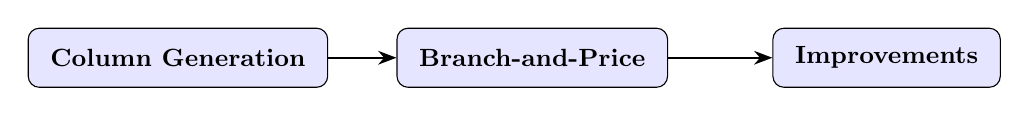
\begin{tikzpicture}[
  box/.style={draw, rounded corners, fill=blue!10,
              minimum height=0.75cm, font=\small\bfseries, inner xsep=8pt},
  arr/.style={-{Stealth}, thick}
]
  \node[box] (cg)  at (0, 0)   {Column Generation};
  \node[box] (bp)  at (4.5, 0) {Branch-and-Price};
  \node[box] (bpc) at (9.0, 0) {Improvements};
  \draw[arr] (cg)  -- (bp);
  \draw[arr] (bp)  -- (bpc);
\end{tikzpicture}
\end{center}
\end{frame}

% ---------------------------------------------------------
% Frame 8: Column Generation Loop
% ---------------------------------------------------------
\begin{frame}{Column Generation}
\begin{center}
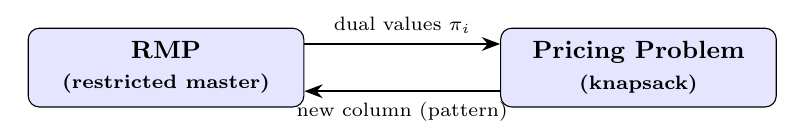
\begin{tikzpicture}[
  box/.style={draw, rounded corners, fill=blue!10, minimum width=3.5cm,
              minimum height=1cm, font=\small\bfseries, align=center},
  arr/.style={-{Stealth}, thick}
]
  \node[box] (rmp) at (0,0) {RMP\\{\scriptsize(restricted master)}};
  \node[box] (pp)  at (6,0) {Pricing Problem\\{\scriptsize(knapsack)}};

  \draw[arr, transform canvas={yshift=3mm}]
    (rmp) -- node[above, font=\scriptsize] {dual values $\pi_i$} (pp);
  \draw[arr, transform canvas={yshift=-3mm}]
    (pp) -- node[below, font=\scriptsize] {new column (pattern)} (rmp);
\end{tikzpicture}
\end{center}

\medskip
\begin{enumerate}
  \item Solve RMP (LP relaxation with a small subset $\mathcal{P}' \subseteq \mathcal{P}$)
  \item Get dual values $\pi_i$ for each covering constraint
  \item Solve pricing problem: find pattern with most negative reduced cost
  \item If reduced cost $\ge 0$: LP optimal. Else: add pattern to $\mathcal{P}'$, go to 1.
\end{enumerate}
\end{frame}

% ---------------------------------------------------------
% Frame 9: RMP and Initial Columns
% ---------------------------------------------------------
\begin{frame}{Restricted Master Problem}
The RMP uses only a \textbf{subset} $\mathcal{P}' \subseteq \mathcal{P}$ of patterns:

\begin{align*}
  \min \quad & \sum_{p \in \mathcal{P}'} z_p \\
  \text{s.t.} \quad
    & \sum_{p \in \mathcal{P}'} a_i^p\, z_p = 1 && \forall\, i \in \mathcal{I} \quad (\pi_i) \\
    & 0 \le z_p \le 1 && \forall\, p \in \mathcal{P}'
\end{align*}

\medskip
\textbf{Initial columns:} We need the RMP to be feasible from the start.

Simplest option: one item per pattern (each item alone in a bin).

\medskip
\begin{center}
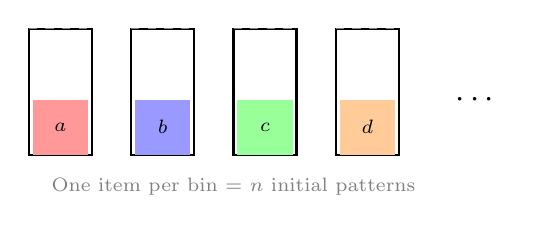
\begin{tikzpicture}[
  bin/.style={draw, thick},
  item/.style={font=\scriptsize\bfseries}
]
  \def\caph{1.6}
  \def\bw{0.8}

  \foreach \i/\col/\lbl [count=\n from 0] in {0/red!40/a, 1/blue!40/b, 2/green!40/c, 3/orange!40/d} {
    \pgfmathsetmacro{\xoff}{\n * 1.3}
    \draw[thick] (\xoff,0) rectangle (\xoff+\bw,\caph);
    \fill[\col] (\xoff+0.05,0) rectangle (\xoff+\bw-0.05, 0.7);
    \node[item] at (\xoff+\bw/2, 0.35) {$\lbl$};
    \draw[dashed, gray] (\xoff,\caph) -- (\xoff+\bw,\caph);
  }

  \node[font=\large] at (5.7, 0.7) {$\cdots$};
  \node[font=\scriptsize, gray] at (2.6, -0.4) {One item per bin = $n$ initial patterns};
\end{tikzpicture}
\end{center}
\end{frame}

% ---------------------------------------------------------
% Frame 10: Exercise --- Initial Columns
% ---------------------------------------------------------
\begin{frame}{Exercise: Initial Columns}
\begin{block}{Task}
Populate the RMP with initial columns using the one-item-per-bin approach:
for each item, create a pattern containing only that item.
\end{block}
\begin{itemize}
  \item File: \texttt{branch\_and\_price/initial\_columns.py}
  \item Test: \texttt{cd branch\_and\_price \&\& python test\_initial\_columns.py}
\end{itemize}

\medskip
\begin{block}{Hint}
Each initial pattern $p_i$ has $a_i^{p_i} = 1$ and $a_j^{p_i} = 0$ for $j \neq i$.
This gives a trivial feasible solution using $n$ bins.
\end{block}
\end{frame}

% ---------------------------------------------------------
% Frame 11: Pricing = Knapsack
% ---------------------------------------------------------
\begin{frame}{Pricing Problem = Knapsack}
Reduced cost of a new pattern $a$:
\[
  \bar{c} = \underbrace{1}_{\text{obj.\ coefficient}} - \underbrace{\sum_{i \in \mathcal{I}} a_i \pi_i}_{\text{column coeffs.\ $\times$ duals}}
\]

Minimize reduced cost subject to bin capacity:
\begin{align*}
  \min \quad & 1 - \sum_{i} a_i\, \pi_i \\
  \text{s.t.} \quad
    & \sum_{i} s_i\, a_i \le C \\
    & a_i \in \{0,1\}
\end{align*}

\pause
$= 1 + \min \left(-\sum_i a_i \pi_i\right) = 1 - \max \sum_i a_i \pi_i \;\;\Rightarrow\;\;$ \textbf{0--1 Knapsack!}

\medskip
When optimal reduced cost $\ge 0$: no improving pattern exists $\Rightarrow$ LP solved.
\end{frame}

% ---------------------------------------------------------
% Frame 12: Pricing in SCIP's Solving Loop
% ---------------------------------------------------------
\begin{frame}{Where Does Pricing Fit in SCIP?}
\begin{center}
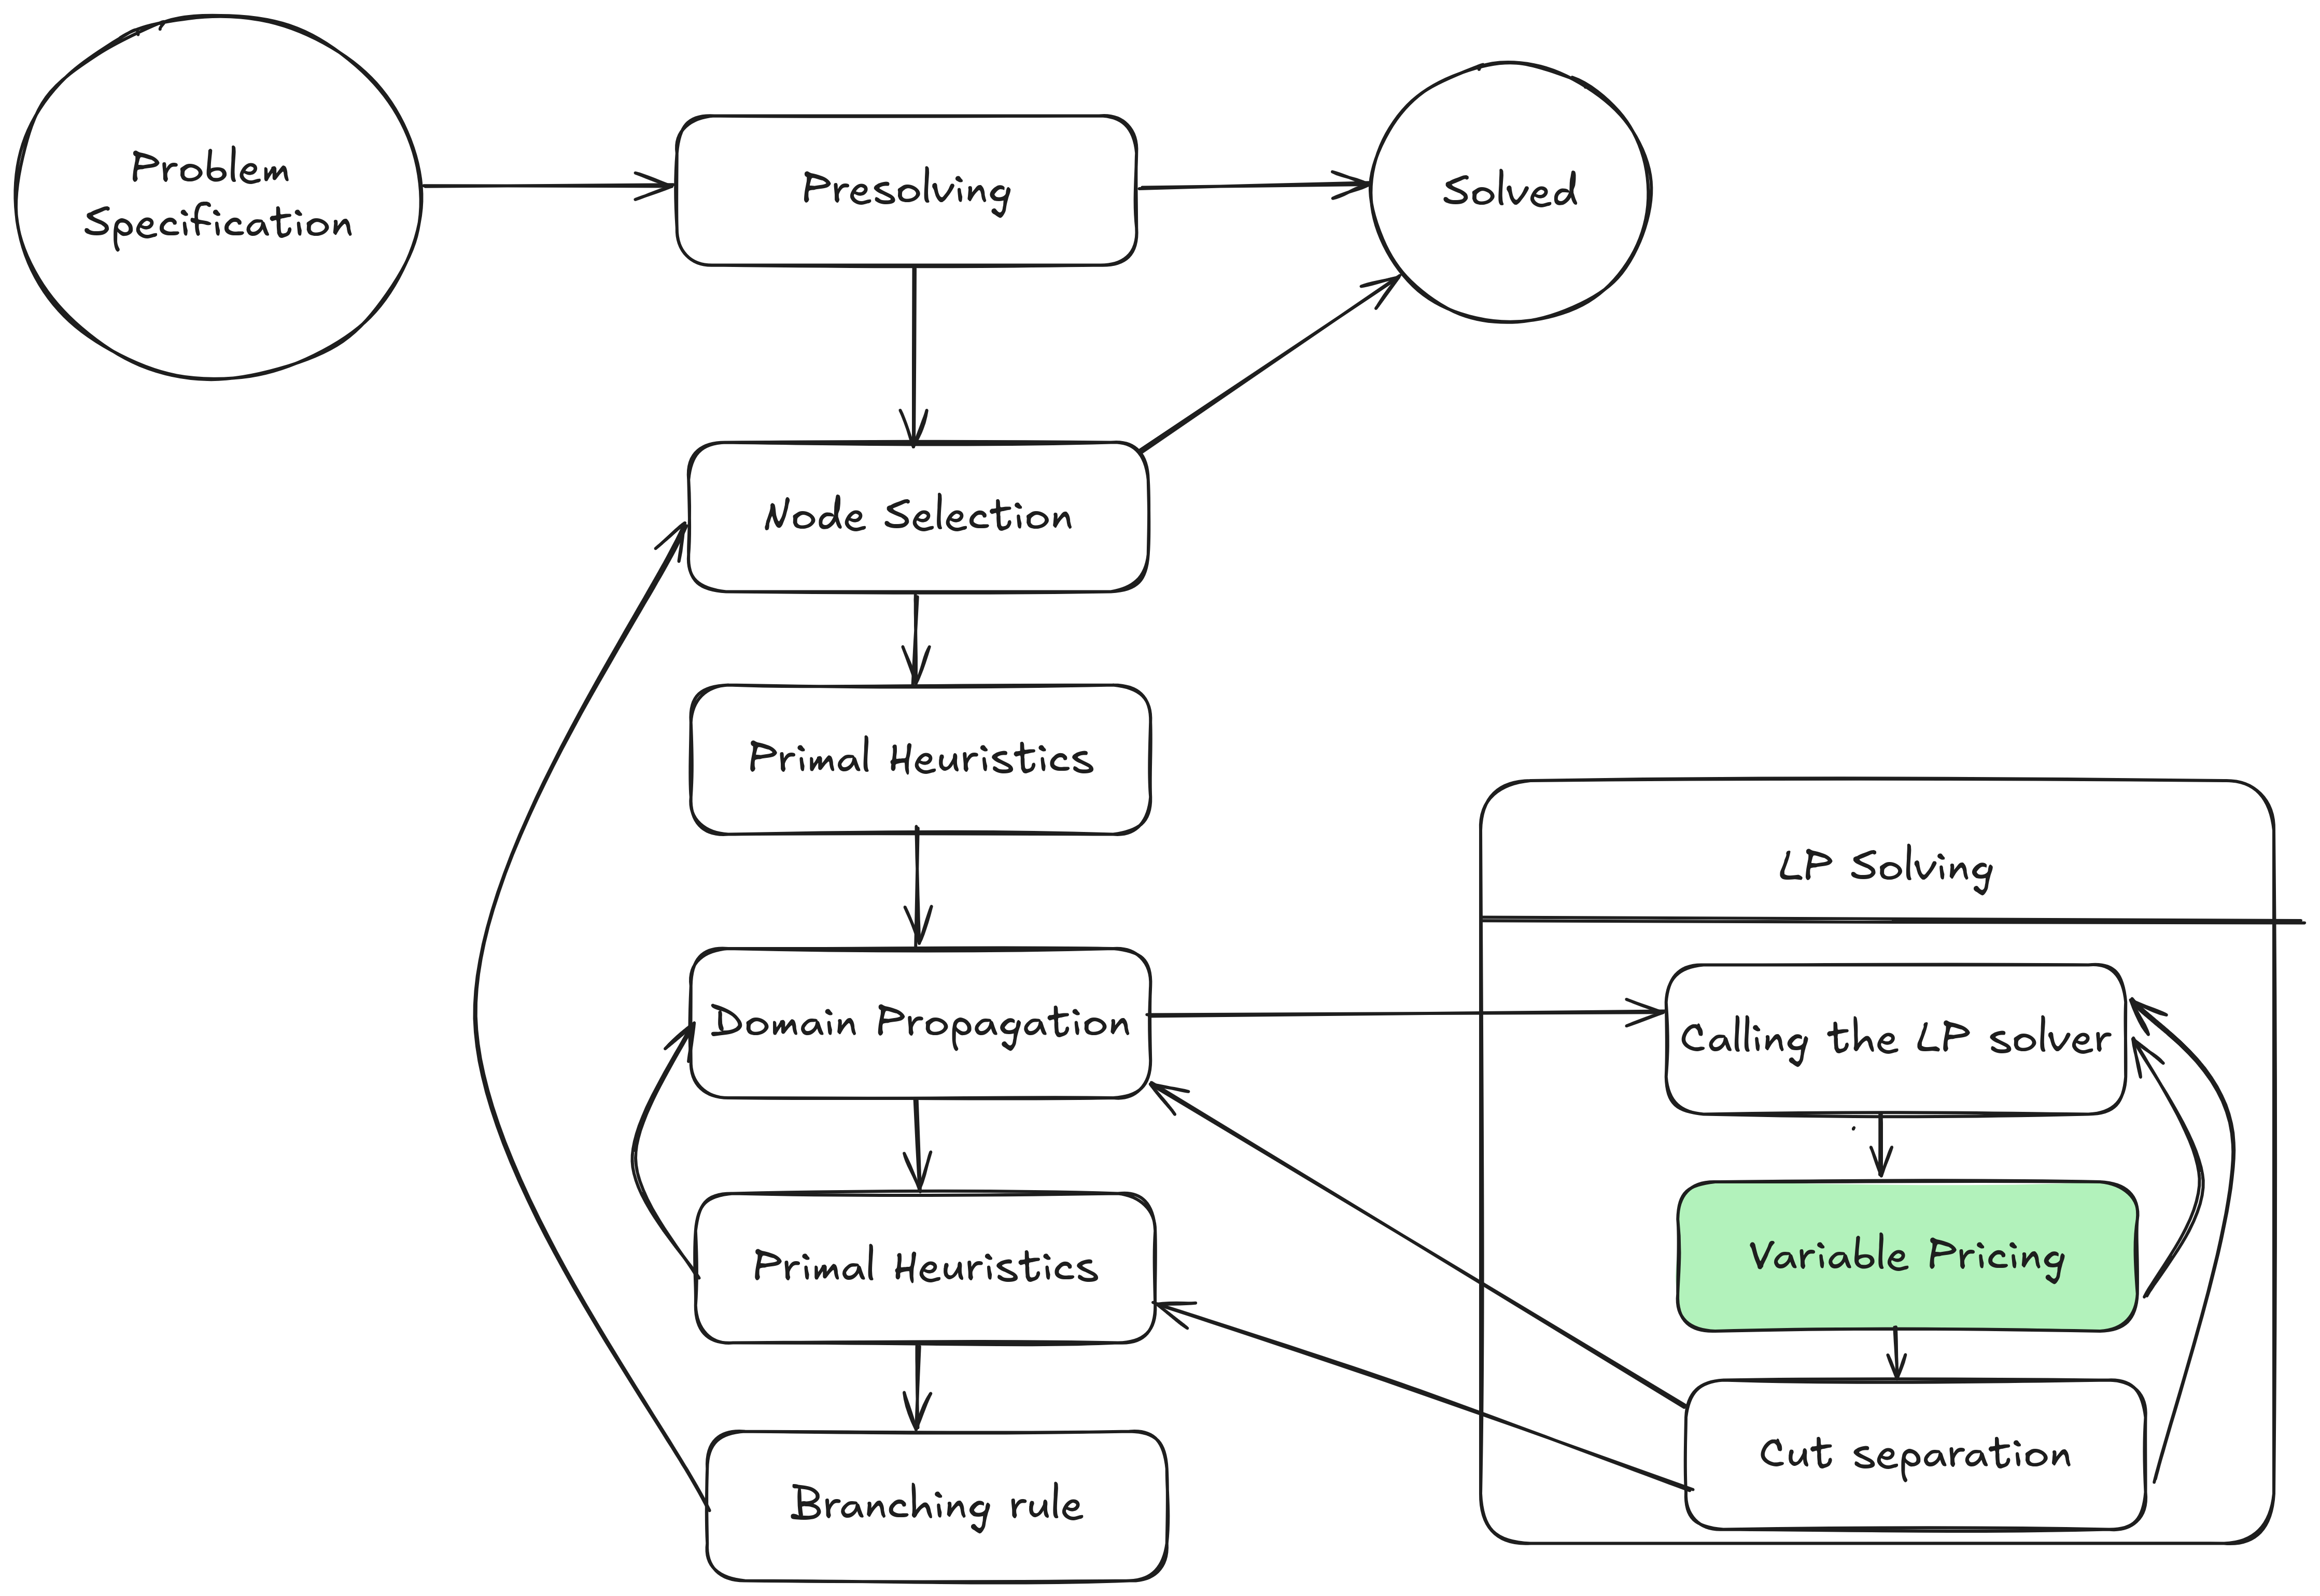
\includegraphics[height=0.55\textheight]{media/scip_solving_loop_pricing.png}
\end{center}

\begin{itemize}
  \item After solving the LP, SCIP calls the \textbf{pricer} plugin
  \item The pricer adds columns with negative reduced cost
  \item LP is re-solved until no improving columns exist
\end{itemize}
\end{frame}

% ---------------------------------------------------------
% Frame 13: Pricer Plugin
% ---------------------------------------------------------
\begin{frame}[fragile]{Pricer Plugin in SCIP}
\begin{table}
\centering\small
\begin{tabular}{lp{8cm}}
\toprule
\textbf{Callback} & \textbf{Purpose} \\
\midrule
\texttt{pricerredcost} & Generate columns with negative reduced cost \\
\texttt{pricerfarkas}  & Generate columns to restore feasibility \\
\bottomrule
\end{tabular}
\end{table}

\medskip
\begin{lstlisting}
class KnapsackPricer(Pricer):
    def pricerredcost(self):
        duals = {i: self.model.getDualsolLinear(cons)
                 for i, cons in self.constraints.items()}
        red_cost, pattern = solve_knapsack(...)
        if red_cost < -1e-6:
            new_var = self.model.addVar(
                vtype="B", obj=1, pricedVar=True)
            # Add coefficients to covering constraints
        return {"result": SCIP_RESULT.SUCCESS}
\end{lstlisting}
\end{frame}

% ---------------------------------------------------------
% Frame 14: Exercise --- Pricing
% ---------------------------------------------------------
\begin{frame}{Exercise: Knapsack Pricing}
\begin{block}{Task}
Implement the 0--1 knapsack solver used as the pricing subproblem.
Return \texttt{(optimal\_value, list\_of\_selected\_items)}.
\end{block}
\begin{itemize}
  \item File: \texttt{branch\_and\_price/pricing\_knapsack.py}
  \item Test: \texttt{cd branch\_and\_price \&\& python test\_pricing\_knapsack.py}
\end{itemize}
\end{frame}

% ---------------------------------------------------------
% Frame 15: Getting Integer Solutions
% ---------------------------------------------------------
\begin{frame}{Getting Integer Solutions}
Column generation solves the \textbf{LP relaxation}. To get integer solutions,
we embed it in \textbf{branch-and-bound}:

\begin{center}
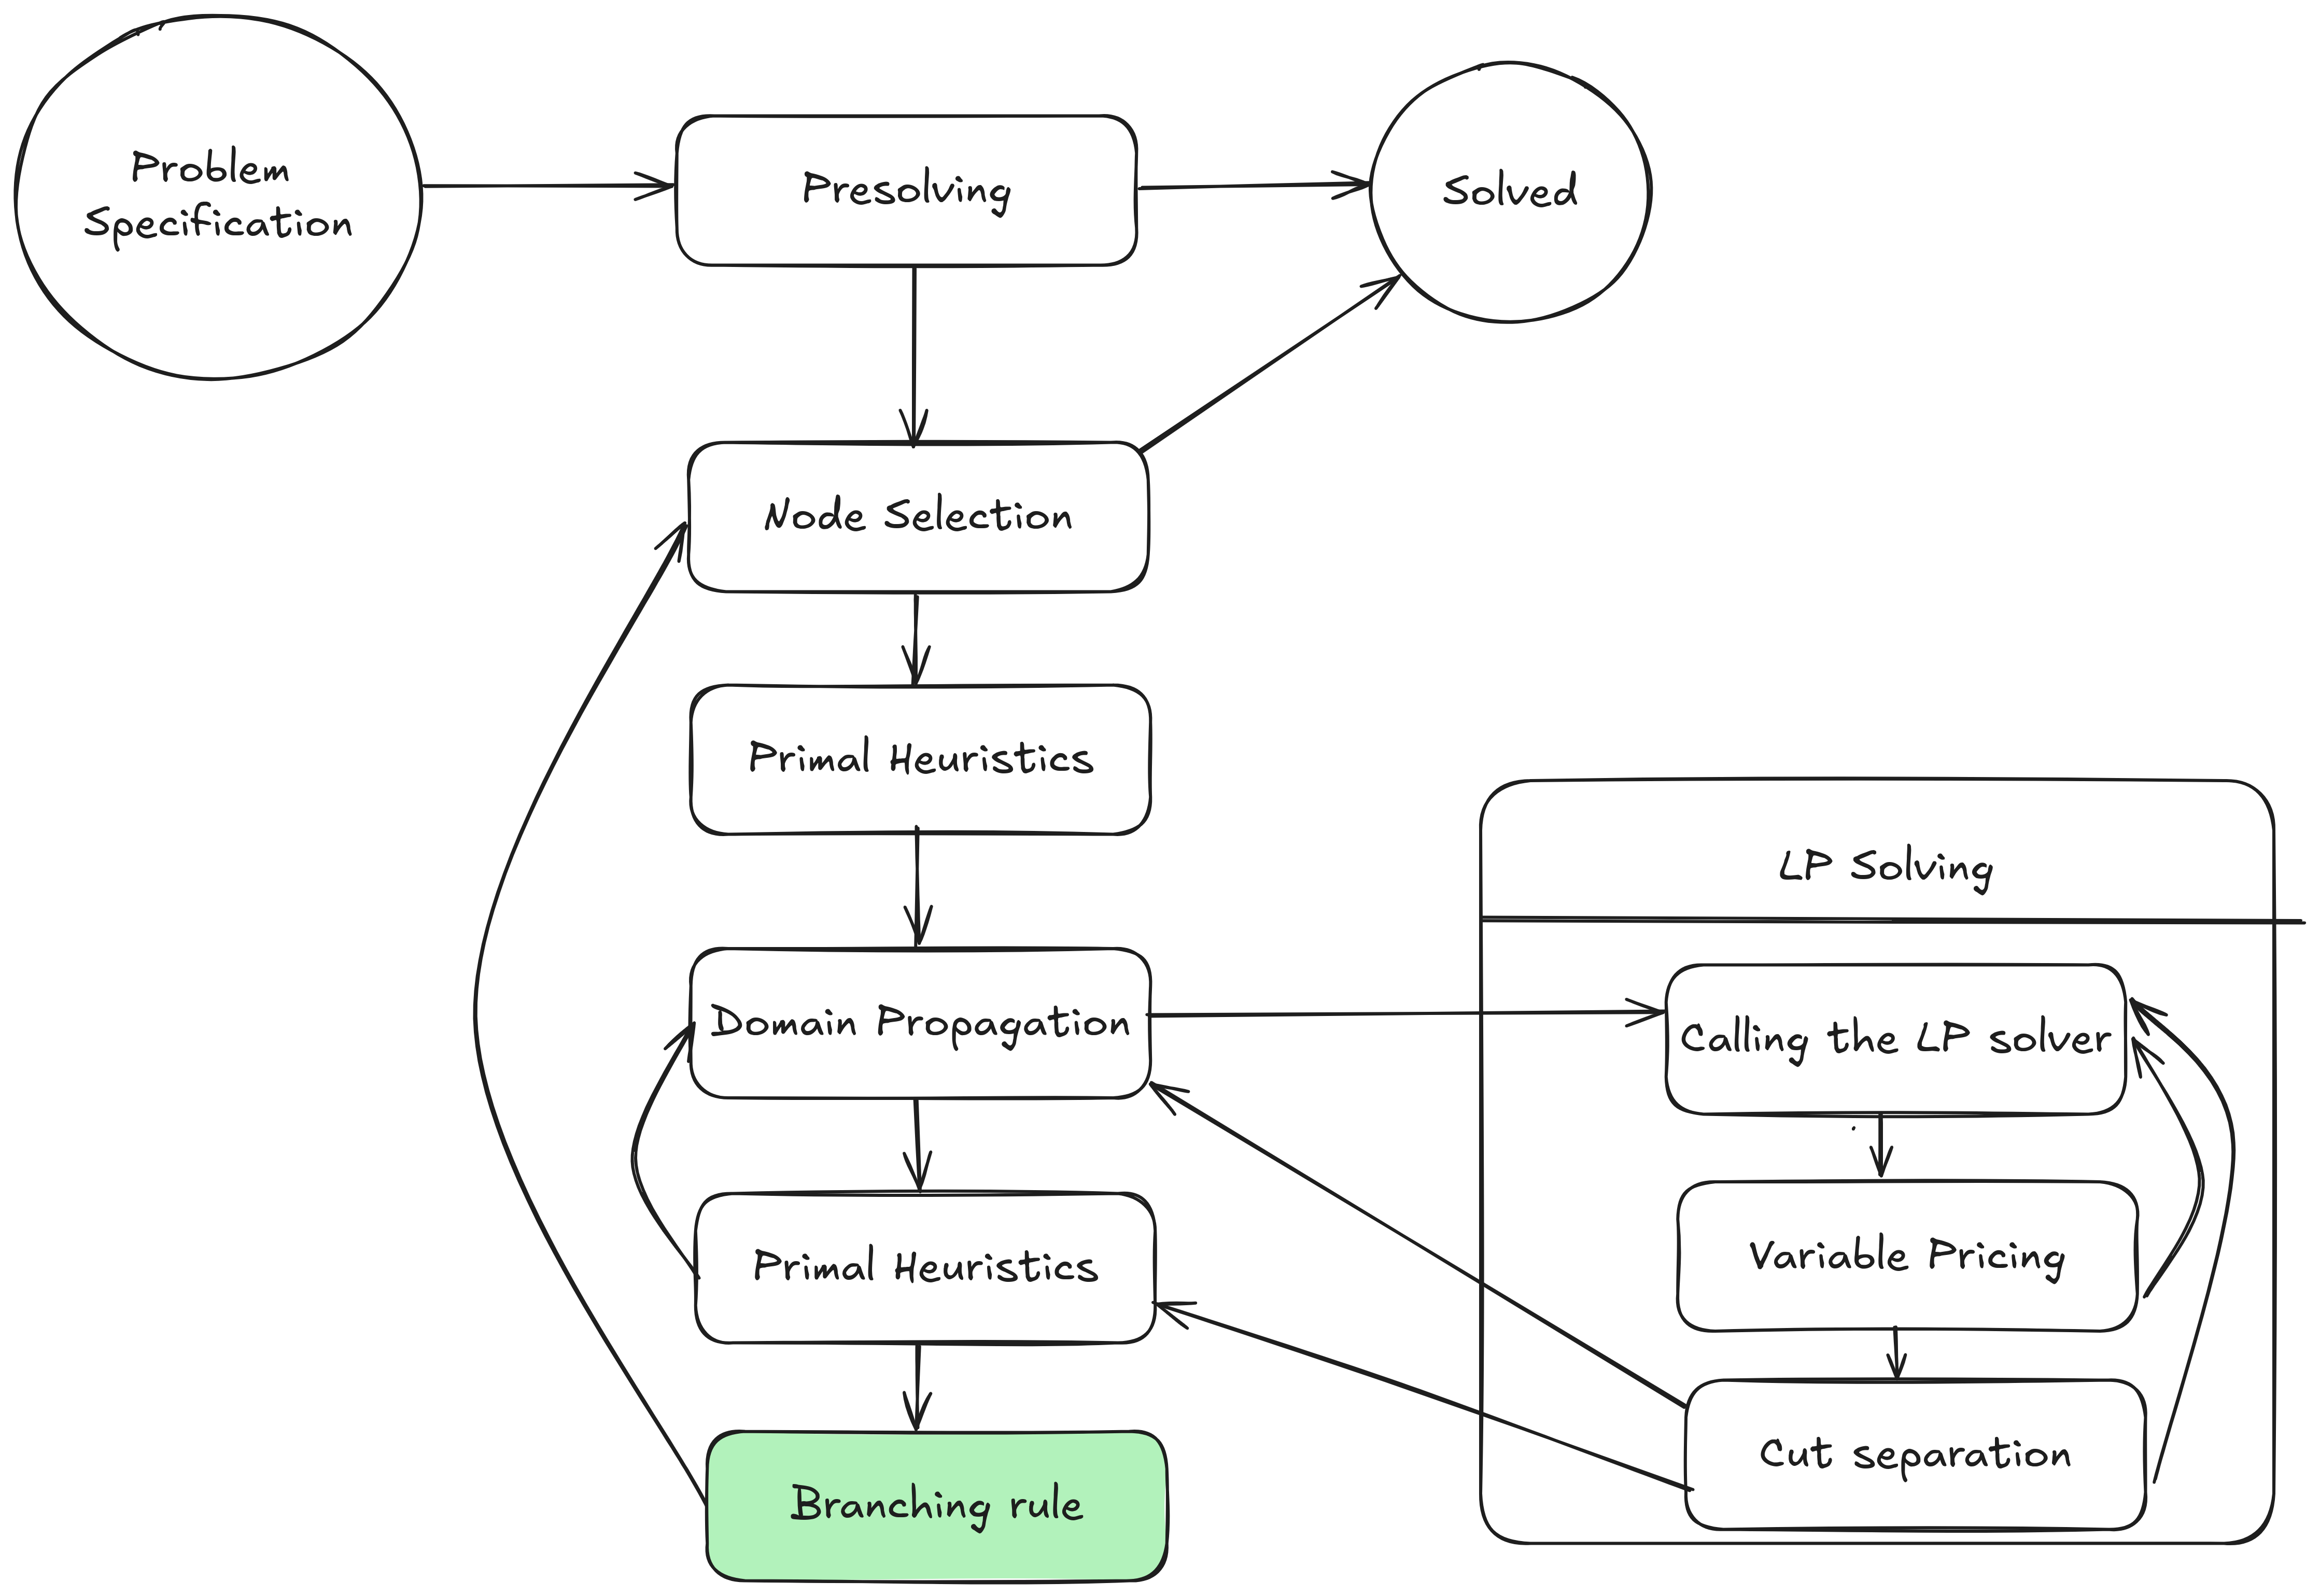
\includegraphics[height=0.55\textheight]{media/scip_solving_loop_branching.png}
\end{center}

\begin{itemize}
  \item At each node: solve LP with column generation
  \item If LP solution is fractional: \textbf{branch}
  \item But \emph{how} should we branch?
\end{itemize}
\end{frame}

% ---------------------------------------------------------
% Frame 16: Why Standard Branching Fails
% ---------------------------------------------------------
\begin{frame}{Why Standard Branching Fails}
Standard variable branching on $z_p$:

\medskip
\begin{columns}[T]
\begin{column}{0.48\textwidth}
\begin{block}{$z_p = 1$}
Force \emph{one specific} packing out of exponentially many.

$\Rightarrow$ \textbf{Very restrictive}
\end{block}
\end{column}
\begin{column}{0.48\textwidth}
\begin{block}{$z_p = 0$}
Forbid \emph{one specific} packing out of exponentially many.

$\Rightarrow$ \textbf{Barely restrictive}
\end{block}
\end{column}
\end{columns}

\bigskip
\begin{center}
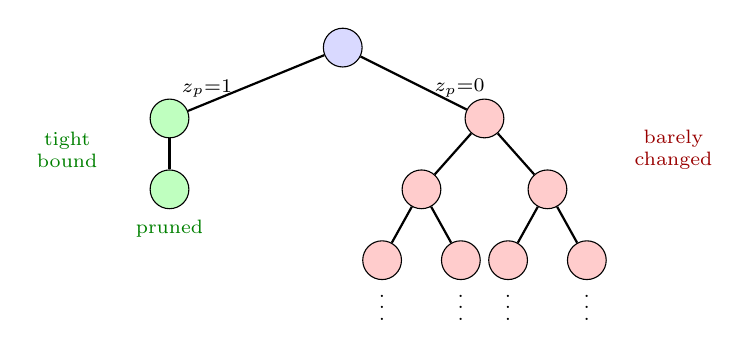
\begin{tikzpicture}[
  nd/.style={circle, draw, fill=blue!15, inner sep=0pt,
             minimum size=14pt, font=\scriptsize},
  lbl/.style={font=\scriptsize, midway},
  edge/.style={thick},
  level distance=0.9cm,
  sibling distance=1.2cm
]
  % Root
  \node[nd] (root) at (0,0) {};

  % Left child: z_p = 1 (deep skinny branch)
  \node[nd, fill=green!25] (l1) at (-2.2, -0.9) {};
  \draw[edge] (root) -- (l1) node[lbl, left, pos=0.6] {$z_p{=}1$};

  % Left subtree - pruned quickly
  \node[nd, fill=green!25] (l2) at (-2.2, -1.8) {};
  \draw[edge] (l1) -- (l2);
  \node[font=\scriptsize, green!50!black] at (-2.2, -2.3) {pruned};

  % Right child: z_p = 0 (deep unbalanced)
  \node[nd, fill=red!20] (r1) at (1.8, -0.9) {};
  \draw[edge] (root) -- (r1) node[lbl, right, pos=0.6] {$z_p{=}0$};

  % Right subtree - keeps going deep
  \node[nd, fill=red!20] (r2) at (1.0, -1.8) {};
  \node[nd, fill=red!20] (r3) at (2.6, -1.8) {};
  \draw[edge] (r1) -- (r2);
  \draw[edge] (r1) -- (r3);

  \node[nd, fill=red!20] (r4) at (0.5, -2.7) {};
  \node[nd, fill=red!20] (r5) at (1.5, -2.7) {};
  \draw[edge] (r2) -- (r4);
  \draw[edge] (r2) -- (r5);

  \node[nd, fill=red!20] (r6) at (2.1, -2.7) {};
  \node[nd, fill=red!20] (r7) at (3.1, -2.7) {};
  \draw[edge] (r3) -- (r6);
  \draw[edge] (r3) -- (r7);

  % Dots indicating more
  \node[font=\scriptsize] at (0.5, -3.2) {$\vdots$};
  \node[font=\scriptsize] at (1.5, -3.2) {$\vdots$};
  \node[font=\scriptsize] at (2.1, -3.2) {$\vdots$};
  \node[font=\scriptsize] at (3.1, -3.2) {$\vdots$};

  % Labels
  \node[font=\scriptsize, green!50!black, align=center] at (-3.5, -1.3)
    {tight\\bound};
  \node[font=\scriptsize, red!60!black, align=center] at (4.2, -1.3)
    {barely\\changed};
\end{tikzpicture}

\smallskip
Result: \textbf{highly unbalanced} tree $\Rightarrow$ very slow convergence
\end{center}
\end{frame}

% ---------------------------------------------------------
% Frame 17: Ryan-Foster Branching
% ---------------------------------------------------------
\begin{frame}{Ryan-Foster Branching}
Branch on \textbf{pairs of items} $(i, j)$ instead of individual variables:

\medskip
\begin{columns}[T]
\begin{column}{0.48\textwidth}
\begin{block}{Together}
Items $i$ and $j$ must be in the \textbf{same} bin.
\end{block}
\end{column}
\begin{column}{0.48\textwidth}
\begin{block}{Apart}
Items $i$ and $j$ must be in \textbf{different} bins.
\end{block}
\end{column}
\end{columns}

\medskip
\begin{columns}[T]
\begin{column}{0.50\textwidth}
\textbf{How to find a pair:}
\begin{itemize}
  \item Compute implicit pair variable: $x_{ij} = \sum_{p:\, i \in p,\, j \in p} z_p$
  \item Choose pair where $0 < x_{ij} < 1$ (fractional)
\end{itemize}

\medskip
$\Rightarrow$ Much more \textbf{balanced} search tree
\end{column}
\begin{column}{0.47\textwidth}
\centering
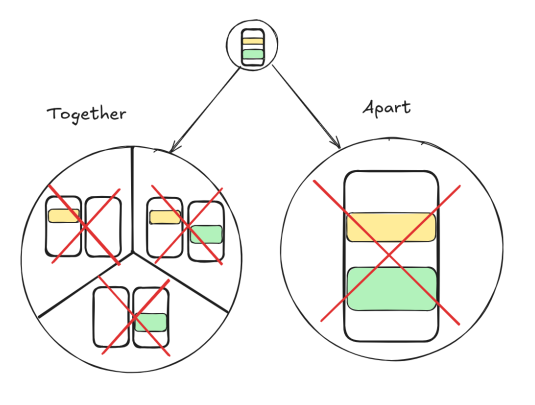
\includegraphics[width=\linewidth]{media/ryan_foster.png}
\end{column}
\end{columns}
\end{frame}

% ---------------------------------------------------------
% Frame 18: Exercise --- Ryan-Foster
% ---------------------------------------------------------
\begin{frame}{Exercises: Ryan-Foster Branching}
\begin{block}{Exercise: Fractional Pairs}
Implement \texttt{all\_fractional\_pairs()} --- find all item pairs with fractional implicit values.
\end{block}
\begin{itemize}
  \item File: \texttt{branch\_and\_price/ryan\_foster.py}
  \item Test: \texttt{cd branch\_and\_price \&\& python test\_fractional\_pairs.py}
\end{itemize}

\medskip
\begin{block}{Exercise: Branching Decisions}
Complete the child-node creation logic: inherit parent decisions, add new pair.
\end{block}
\begin{itemize}
  \item File: \texttt{branch\_and\_price/ryan\_foster.py}
\end{itemize}
\end{frame}

% ---------------------------------------------------------
% Frame 19: Enforcing Branching in Pricing
% ---------------------------------------------------------
\begin{frame}[fragile]{Enforcing Branching in Pricing}
The pricing problem must respect \textbf{all} accumulated branching decisions:

\medskip
\begin{itemize}
  \item \textbf{Together} $(i, j)$: add constraint $a_i = a_j$ in knapsack
  \item \textbf{Apart} $(i, j)$: add constraint $a_i + a_j \le 1$ in knapsack
\end{itemize}

\medskip
\begin{lstlisting}
# Together constraints
for i, j in together:
    m.addCons(x[i] == x[j])

# Apart constraints
for i, j in apart:
    m.addCons(x[i] + x[j] <= 1)
\end{lstlisting}

\end{frame}

% ---------------------------------------------------------
% Frame 20: Exercise --- Constrained Pricing
% ---------------------------------------------------------
\begin{frame}{Exercise: Constrained Pricing}
\begin{block}{Task}
Implement \texttt{solve\_knapsack\_with\_constraints()} --- extend the knapsack solver
with together/apart constraints from Ryan-Foster branching.
\end{block}
\begin{itemize}
  \item File: \texttt{branch\_and\_price/pricing\_knapsack.py}
  \item Test: \texttt{cd branch\_and\_price \&\& python test\_knapsack\_with\_constraints.py}
\end{itemize}

\medskip
\begin{block}{Integration Test}
After all B\&P exercises: \texttt{cd branch\_and\_price \&\& python test\_bnp.py}
\end{block}
\end{frame}

% ---------------------------------------------------------
% Frame 21: Branch-Price-and-Cut
% ---------------------------------------------------------
\begin{frame}{Branch-Price-and-Cut}
Strengthen branch-and-price by adding \textbf{cutting planes}.

\medskip
\textbf{Subset-row inequalities} for set partitioning:

For any triple of items $S = \{i, j, k\}$, consider all packings covering
$\ge 2$ items in $S$. If their LP values sum $> 1$:
\[
  \sum_{p:\, |p \cap S| \ge 2} z_p \le 1
\]

\medskip
\textbf{Separator plugin} in SCIP:
\begin{itemize}
  \item \texttt{sepaexeclp}: search for violated inequalities at each LP solution
  \item Return \texttt{SEPARATED} if cut added, \texttt{DIDNOTFIND} otherwise
\end{itemize}
\end{frame}

% ---------------------------------------------------------
% Frame 22: Exercise --- Subset-Row Separator
% ---------------------------------------------------------
\begin{frame}{Exercise: Subset-Row Separator}
\begin{block}{Task}
Implement the subset-row separator: enumerate triples of fractional
LP variables and add cuts when their values sum exceeds 1.
\end{block}
\begin{itemize}
  \item File: \texttt{separator/subset\_row/subset\_row.py}
  \item Test: \texttt{cd separator/subset\_row \&\& python test\_subset\_row.py}
\end{itemize}
\end{frame}

% ---------------------------------------------------------
% Frame 23: Summary
% ---------------------------------------------------------
\begin{frame}{Summary \& Further Resources}
\textbf{What we covered:}
\begin{itemize}
  \item Bin packing: compact vs.\ extended formulation
  \item Column generation with knapsack pricing
  \item Branch-and-price with Ryan-Foster branching
  \item Branch-price-and-cut with subset-row inequalities
\end{itemize}

\medskip
\textbf{Bonus exercises} (see \texttt{branch\_and\_price/README.md}):
\begin{itemize}
  \item Dual stabilization, Lagrangian bound
  \item Better initialization, faster pricing
  \item Handling numerical issues
\end{itemize}

\medskip
\textbf{Resources:}
\begin{itemize}
  \item \url{https://www.scipopt.org/} --- SCIP documentation
  \item \url{https://github.com/scipopt/PySCIPOpt} --- PySCIPOpt
\end{itemize}
\end{frame}

\end{document}
